\documentclass[border=10pt]{standalone}
\usepackage{tikz}
\usetikzlibrary{arrows.meta, shapes, positioning}

\begin{document}
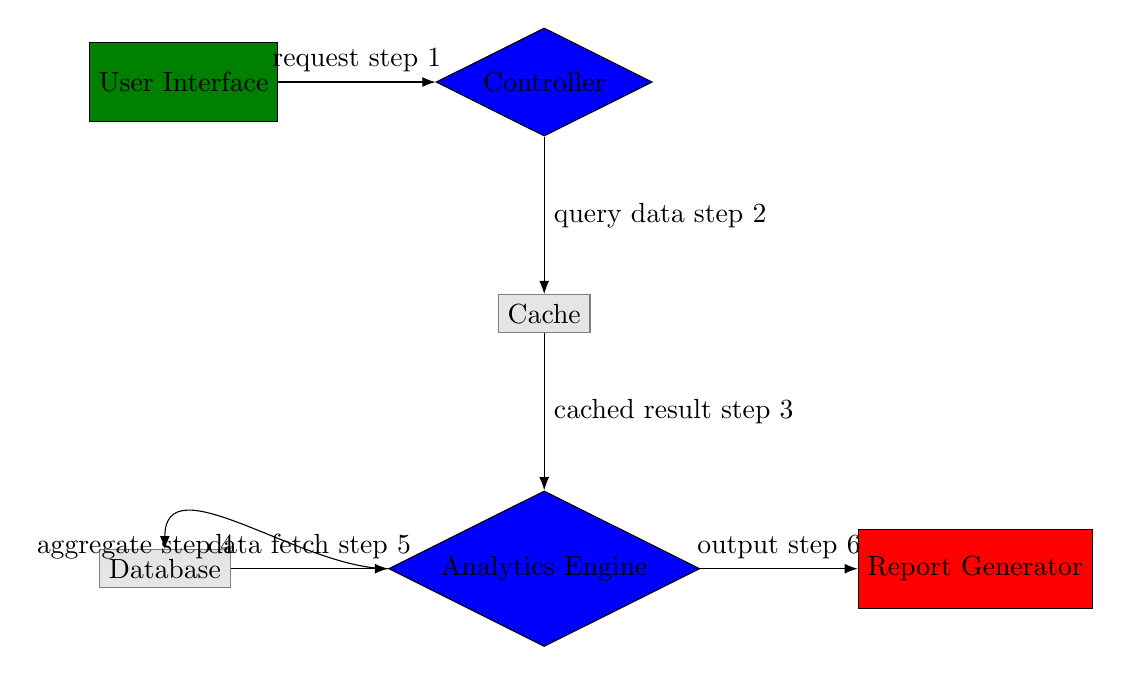
\begin{tikzpicture}[node distance=2cm, auto,
    rect/.style={rectangle, draw, fill=#1, minimum width=2cm, minimum height=1cm},
    diam/.style={diamond, draw, fill=#1, aspect=2, minimum width=2cm, minimum height=1cm},
    arrow/.style={->, >=Latex}
]

% Nodes
\node[rect=green!50!black] (ui) {User Interface};
\node[diam=blue] (ctrl) [right=of ui] {Controller};
\node[draw=gray, fill=gray!20] (cache) [below=of ctrl] {Cache};
\node[diam=blue] (ae) [below=of cache] {Analytics Engine};
\node[rect=red] (rg) [right=of ae] {Report Generator};
\node[draw=gray, fill=gray!20] (db) [left=of ae] {Database};

% Arrows and Labels
\draw[arrow] (ui) -- node {request step 1} (ctrl);
\draw[arrow] (ctrl) -- node {query data step 2} (cache);
\draw[arrow] (cache) -- node {cached result step 3} (ae);
\draw[arrow] (ae) -- node {output step 6} (rg);
\draw[arrow] (db) -- node {data fetch step 5} (ae);
\draw[arrow] (ae) to[out=180,in=90] node {aggregate step 4} (db);

\end{tikzpicture}
\end{document}